\documentclass{article}
\usepackage{graphicx}
\usepackage[margin=1.5cm]{geometry}
\usepackage{amsmath}

\begin{document}

\title{Midterm 1: Elementary Statistics}
\author{Prof. Jordan C. Hanson}

\maketitle

\section{Formula Area}

\begin{enumerate}
\item Quantitative continuous data: sample data that can be measured
\item Quantitative discrete data: sample data that can be counted
\item Qualitative or categorical data: sample data that can be classified but not counted
\item Average/mean, definition 1: $\bar{x} = N^{-1} \sum_i x_i$ for a sample size $N$
\item Median: the value below which are half of the frequencies.  Half of the frequencies are also above this value.
\item Mode: the value corresponding to the highest frequendy.
\item The quartiles $Q1$, $Q2$, and $Q3$ are the values that separate the frequencies into four bins of equal frequency. $Q2$ is equal to the median.  The IQR is $Q3 - Q1$.
\item The k-th percentile: the value below which k percent of the data is located.  Formula: $i = (k/100) (n+1)$, where $k$ is the percentile, $n$ is the total number of data, and $i$ is the integer location of the k-th percentile.
\item Finding the percentile of a data value: $(x+0.5*y)/n (100)$, where $x$ is the number of data values below the given data value, $y$ is the number of data values equal to the given one, and $n$ is the total number of data values.
\item Average/mean, definition 2: $\bar{x} = \sum_i^{M} f_{r,i} x_i$, where $x_i$ are the bin centers of a histogram, or the discrete random variable data values, $M$ is the number of bins, and $f_{r,i}$ are the relative frequencies.  For a discrete random variable, $f_{r,i}$ is replaced with $p(x)$, the probability distribution function.
\item Probabilities of mutually exclusive and independent events: if two events have probabilities $p_1$ and $p_2$, then the probability that event 1 AND event 2 occur is $p_1 p_2$.  The probability that event 1 OR event 2 occurs is $p_1 + p_2$.
\item The standard deviation $s$ of a sample of size $N$ is 
\begin{equation}
s^2 = \frac{1}{N-1}\sum_{i=1}^N (x_i-\mu)^2
\end{equation}
\item Mean or expectation value of a binomial distribution: $\mu = Np$
\item Standard deviation of a binomial distribution: $\sigma = sqrt{N p (1-p)}$
\end{enumerate}

\clearpage

\section{Unit 0}

\begin{enumerate}
\item Suppose we measure 10 resting heart rates from 10 college students...during finals, and they've each had coffee.  We find: 59, 60, 70, 75, 75, 75, 76, 77, 77, and 78 beats per minute.  Provide the following:
\begin{itemize}
\item What is the sample size?
\item What is the mean heart rate?
\item What is the standard deviation of the heart rates?
\item Describe one issue with the sample that affects its randomness.  How would you get a more complete sample of the student population at Whittier College?
\end{itemize}
\vspace{1cm}
\item Whittier College collects data on the number of students that apply each year, and the proportion we accept and who enroll.  See Fig. \ref{fig:admit}, and copy the data into a spreadsheet like LibreOffice Calc or Microsoft Excel.
\begin{figure}[ht]
\centering
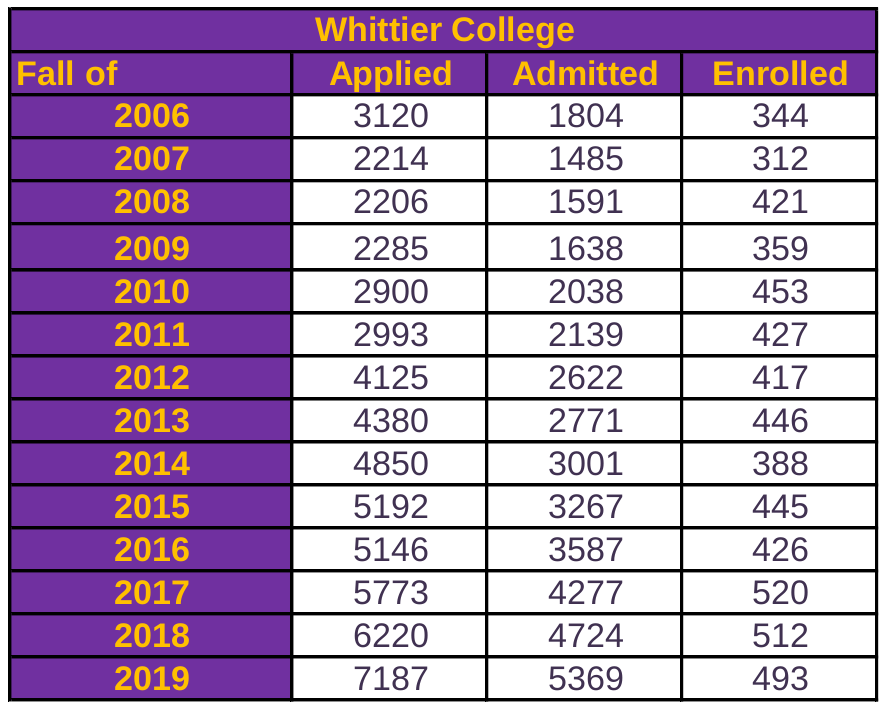
\includegraphics[width=0.35\textwidth]{figures/admit.png}
\caption{\label{fig:admit} A table of the number of freshmen who applied, were accepted, and were enrolled in Whittier College, versus year.}
\end{figure}
\begin{itemize}
\item What is the mean number of newly enrolled freshmen per year from 2006 - 2019?
\item Define the \textit{acceptance rate} as the second column of Fig. \ref{fig:admit} divided by the first.  What is the average acceptance rate from 2006 to 2019?
\item What is the standard deviation of the acceptance rate from 2006 - 2019?  Are there any outliers?
\item Graph the \textit{time-series} of the acceptance rate.
\end{itemize}
\vspace{5cm}
\item In a particular fund, there are 10 stocks, each with the following price per share in USD: 109.00, 108.00, 112.00, 113.00, 113.00, 120.00, 151.00, 170.00, 250.00, and 290.00.  (a) What price represents the 75th percentile? (b) To what percentile does 113.00 dollars correspond? (c) What is the standard deviation and mean of the data? (d) Create a histogram of the data.  Do you notice skew? \\ \vspace{3cm}
\item \textbf{Pirate Dice.} Imagine you are kidnapped by pirates, and to pass the time between scrubbing the deck and serving grog, you wager on dice.  Each of four players has two dice.  Each player rolls his or her dice but hides them from sight after looking at them.  The players take turns stating how many instances of a number will appear among the 8 dice. If any player thinks the claim is false (a lie), then they call \textbf{liar}.  If the player was wrong, they are out. For example, if each pair of dice are: (1,2), (4,4), (4,6), and (3,5), then there are three ``fours'' all together.  Calling four ``fours'' would be a lie.  (a) Your dice say (1,1).  An opponent declares that ``there be \textit{five ones}'' in play.  What is the probability this is true? (b) Your dice say (2,3).  An opponent declars that ``there be \textit{six fives}!'' What is the probability? \\ \vspace{3cm}
\item Consider a \textit{fair coin} where the probability of a heads, P(H), is 0.5, and the probability of a tails, P(T), is 0.5.  Suppose we model the random motion of a gas molecule in 1D like a fair coin, in which movement left by one unit has a probability L = P(T) and movement right by one unit has a probability R = P(H).  (a) What is the probability that a molecule follows this path: LRLLRLRR? (b) What is the probability a molecule follows this path: RRRRRRRR? (c) Which is more common, a path that leads back to the starting point, or the path in part (b)? \\ \vspace{2cm}
\end{enumerate}

\section{Unit 1}

\begin{enumerate}
\item Suppose a stock trader agrees to purchase stock at a future date, according to a contract that stipulates she \textit{must} purchase it, regardless of the price.  However, she negotiates that the price will be measured into one of four bins, the centers of which are shown in Tab. \ref{tab:stock}.  This makes the price a discrete random variable.  She performs an analysis that gives the probability that the stock price will fall into each of the categories.  If she buys one share, what is the \textit{expectation value} of her profit? What would be her profit if she buys 1000 shares?
\begin{table}[hb]
\centering
\begin{tabular}{| c | c | c | c |}
\hline
\textbf{Outcome} & $x$ & $p(x)$ & $x*p(x)$ \\ \hline \hline
Price bin 1 & \$90.00 per share & $0.01$ & ? \\ \hline
Price bin 2 & \$16.00 per share & $0.49$ & ? \\ \hline
Price bin 3 & -\$15.00 per share & $0.49$ & ? \\ \hline
Price bin 4 & -\$95.00 per share & $0.01$ & ? \\ \hline
\hline
\end{tabular}
\caption{\label{tab:stock} A table displaying a stock trader's assessment of the probability a stock will fall into one of four bins. (The bin centers are shown).}
\end{table}
\clearpage
\item Suppose a psychologist is studying whether or not people can decide if another person has an IQ score of greater than 100.  Ten different people are shown ten different images of another person for 2.0 seconds.  So you can think of an individual photo as a trial, and each participant as a run.  The frequencies with which the participants said yes, $IQ > 100$ is shown in Tab. \ref{tab:baby}.  (a) Fill in Tab. \ref{tab:baby}, given what you know about the experiment.  (b) Are the participants guessing randomly?  Why or why not?  (c) Are the data distributed following a binomial distribution?  Assuming they are, what is the $p$ value that satisfies $\mu = Np$?
\begin{table}[ht]
\centering
\begin{tabular}{| c | c | c | c |}
\hline
\textbf{$x$} & $N_{good}$ & $p(x)$ & $x*p(x)$ \\ \hline \hline
0 & 0 &  &  \\ \hline
1 & 0 &  &  \\ \hline
2 & 0 &  &  \\ \hline
3 & 0 &  &  \\ \hline
4 & 1 &  &  \\ \hline
5 & 0 &  &  \\ \hline
6 & 3 &  &  \\ \hline
7 & 6 &  &  \\ \hline
8 & 0 &  &  \\ \hline
9 & 0 &  &  \\ \hline
10 & 0 &  &  \\ \hline
\hline
\end{tabular}
\caption{\label{tab:baby} A table displaying the frequencies with which participants decided random photos of people corresponded to an IQ score of larger than 100 or not.  The left column is the discrete random variable $x$, the total number of times the participant decided a photo corresponding to a high IQ.  The middle column is the frequency with which $x$ occurs across 10 runs.}
\end{table}
\end{enumerate}

\end{document}